\documentclass[12pt,french,dvips]{report} 

\usepackage[utf8]{inputenc}
\usepackage[OT1,T1]{fontenc}
\usepackage{mdframed}
\usepackage{graphicx}
\usepackage{amsmath}
\usepackage{babel}
\usepackage{dcolumn}
\usepackage{tabularx}
\usepackage{colortbl}
\usepackage{lscape}
\usepackage{enumerate,comment,overcite}
\usepackage{pst-spectra}
\usepackage{helvet}
\usepackage{elements}
\usepackage{modiagram}

\graphicspath{{/home/paola/pres/logos/},
              {/home/paola/TEACH/ue13/2015_2016/td/figure/}}

%%% DIMENSION OF THE TEXT
\textwidth = 6.7 in
\textheight = 8.5 in
\oddsidemargin = -0.3in
\evensidemargin = 0.0 in
\topmargin = -.7 in
\headheight = 35 pt
\headsep = 0.0 in
\parskip = 0.2in
\parindent = 0.0in

\newcounter{numTD}
\newtheorem{exercice}{Exercice}
\newtheorem{methodologie}{M\'ethodologie}
\newtheorem{correction}{Correction}
\newcommand{\exo}[1]{\setlength{\parskip}{0.pt}\begin{exercice} \emph{\textbf{- #1}} \end{exercice}}
\newcommand{\meth}[1]{\setlength{\parskip}{0.pt}\begin{methodologie} \emph{\textbf{- #1}} \end{methodologie}}
\newcommand{\sol}[1]{\setlength{\parskip}{0.pt}\begin{correction} \emph{\textbf{- #1}} \end{correction}}
%\newcommand{\pb}[1]{\setlength{\parskip}{0.pt}\begin{probleme} \emph{\textbf{- #1}} \end{probleme}}
%%% commande titre TD
\newcommand{\titreTD}[2]{\addtocounter{numTD}{1}
\begin{center}
\Large\textbf{TD n$^\textrm{\small o}$#1 - #2}
\vspace{0.5cm}
\end{center}
}
\setcounter{secnumdepth}{0}
\renewcommand{\titreTD}[2]{\section{#2}}

\newpsobject{showgrid}{psgrid}{subgriddiv=1,griddots=10,gridlabels=6pt}

\def\thesection{\arabic{section}}

\title{{\Huge Corrections des TRAVAUX DIRIG\'ES  \\[1.5cm] 
\textsl{Atome et Liaison chimique}}}
\author{Portail Curie}

\begin{document}
\section{Modèle de Bohr}
\subsection{Exercice 9}
Il est indiqué que la lumière est due à une réaction chimique que l'on peut écrire~:
\begin{align*}
\text{luciferine} + ATP + n Mg^{2+} \xrightarrow{\text{luciferase}} \text{luciferine oxydée excitée} \rightarrow produits + lumiere
\end{align*}
Il s'agit donc d'un phénomène d'emission: la lumière est émise à la suite de la désexcitation
de la luciférine oxydée.
\subsection{Exercice 10}
Si le verre ne contient que de l'eau, à la lumière du soleil, elle apparaît incolore: l'eau laisse
passer toutes les longueurs d'onde de la lumière visible.
Lorsqu'on mélange de la grenadine à l'eau, elle apparaît rouge: une partie des longueurs
d'ondes visibles ont été absorbées par le colorant contenu dans le sirop.
Dans le cas du colorant rouge se trouvant dans le sirop, il s'agit d'une molécule
qui absorbe toutes les longueurs d'onde sauf celles donnant une couleur rouge: le mélange apparaît rouge.%
\footnote{Dans le cas d'un sirop de menthe, il n'y a pas 1 mais 2 colorant: l'un est bleu, l'autre jaune
ce qui donne un couleur verte au mélange.}
\subsection{Exercice 11}
\begin{enumerate}
\item un hydrogénoïde est composé d'un noyau atomique de charge Z et d'un seul électron: c'est bien le
cas de He$^+$.
\begin{align*}
E_n = -13,6 \frac{Z^2}{n^2}
\end{align*}
\begin{tabular}{lrrrrrrr}\hline
n & 2 & 3 & 4 & 5 & 6 & 7 & 8 \\ \hline \hline
H (eV)  & -3.40  & -1.51 & -0.85 & -0.54 & -0.38 & -0.28 & -0.21 \\
He (eV) & -13.60 & -6.04 & -3.40 & -2.18 & -1.51 & -1.11 & -0.85 \\
H (J)   & -5.44E-19 & -2.42E-19 & -1.36E-19 & -8.70E-20 & -6.04E-20 & -4.44E-20 & -3.40E-20 \\
He (J)  & -2.18E-18 & -9.67E-19 & -5.44E-19 & -3.48E-19 & -2.42E-19 & -1.78E-19 & -1.36E-19 \\
\hline \hline
\end{tabular}\\
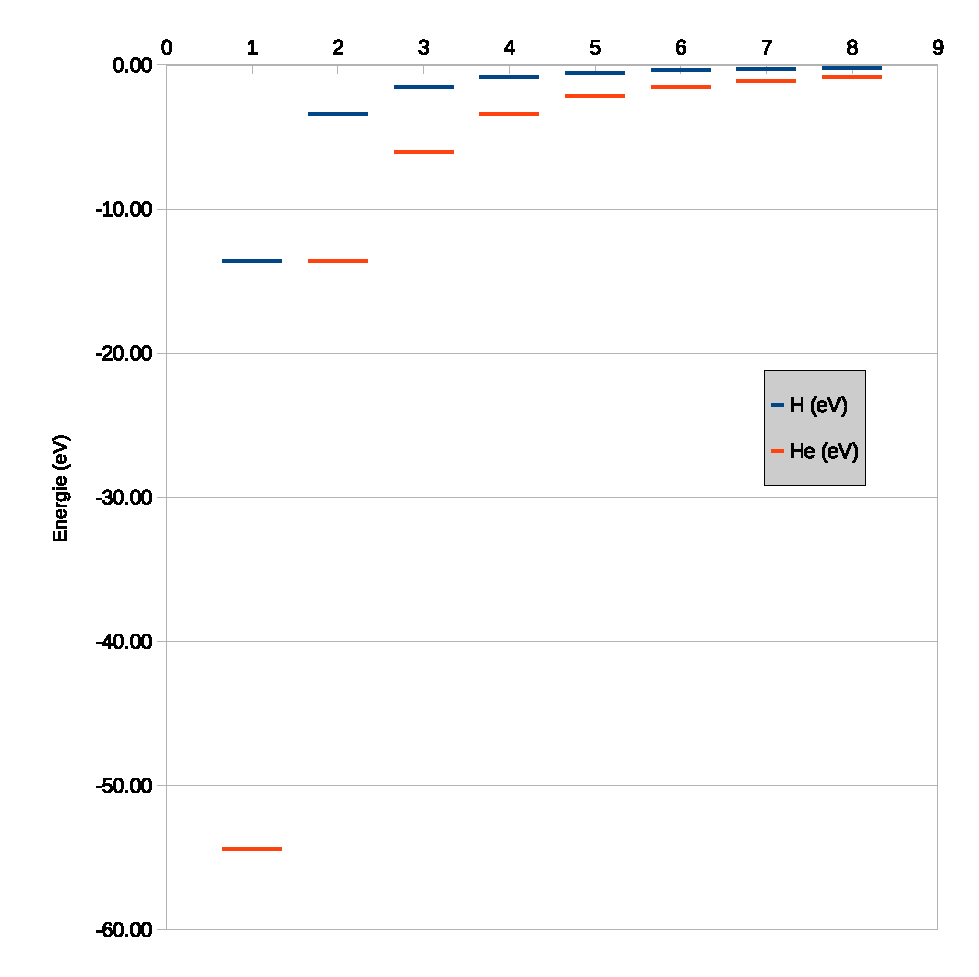
\includegraphics[width=1.0\textwidth]{figure/niveaux.eps}
\item Pour connaître le domaine dans lequel se trouve la série de Lyman, on calcule ses longueurs
d'onde maximales et minimales:\\
Longueur d'onde maximale : $n=2\rightarrow n=1$
\begin{align*}
\Delta E & =  \left|-13.6 ( \frac{1^2}{1^2} - \frac{1^2}{2^2} ) \right| \\
         & = 10.2 eV \\
\lambda_{max} & = \frac{hc}{\Delta E} \\
              & = \frac{6.626\times10^{-34} \times 3\times 10^8}{10.2\times1.602\times10^{-19}}\\
              & = 121,6 nm
\end{align*}
Longueur d'onde minimale : $n=\infty\rightarrow n=1$
\begin{align*}
\Delta E & = \left| -13.6 ( \frac{1^2}{1^2} - 0               ) \right| \\
         & = 13.6 eV \\
\lambda_{max} & = \frac{hc}{\Delta E} \\
              & = \frac{6.626\times10^{-34} \times 3\times 10^8}{13.6\times1.602\times10^{-19}}\\
              & = 91,2 nm
\end{align*}
Toutes les longueurs d'ondes de la série de Lyman se trouvent entre 91,2 et 121,6 nm, elles sont
donc toutes hors du visible.
\begin{itemize}
\item $400nm\rightarrow3,10 eV$
\item $800nm\rightarrow1,55 eV$
\item On calcule toutes les énergies de transition possibles et on cherche celles
qui se trouvent entre 3,10 et 1,55.\\
\begin{tabular}{lrrrrrr}\hline\hline
n & 1 & 2 & 3 & 4 & 5 & 6 \\\hline
He (eV) &-54.4 &-13.6 &-6.0 &-3.4 &-2.2 &-1.5 \\
\hline
$(n+1)\rightarrow n$   && 40.8 & 7.6 & \textbf{2.6} & 1.2 & 0.7 \\
$(n+2)\rightarrow n$&& & 48.4 & 10.2 & 3.9 & \textbf{1.9} \\
$(n+3)\rightarrow n$&& & & 51.0 & 11.4 & 4.5 \\
$(n+4)\rightarrow n$&& & & & 52.2 & 12.1 \\
$(n+5)\rightarrow n$&& & & & & 52.9 \\\hline\hline
\end{tabular}\\
Seules deux transitions sont dans le domaine du visible: $n: 4\rightarrow 3$ et $n: 6\rightarrow 4$
Ce sont des transitions d'un état excité vers un autre: elles sont peu probables donc difficiles
à observer.
\end{itemize}
\item Si on part de n=3 on peut faire les desexcitations suivantes:\\
\begin{tabular}{lll}
chemin 1: & $3\rightarrow 1$ \\
chemin 2: & $3\rightarrow 2$ & $2\rightarrow 1$ \\
\end{tabular}
\end{enumerate}
Il y aura donc 3 raies d'emission.\\
En partant de n=4, on a:\\
\begin{tabular}{llll}
chemin 1: & $4\rightarrow 1$ \\
chemin 2: & $4\rightarrow 2$ & $2\rightarrow 1$ \\
chemin 3: & $4\rightarrow 3$ & $3\rightarrow 1$ \\
chemin 4: & $4\rightarrow 3$ & $3\rightarrow 2$ & $2\rightarrow 1$ \\
\end{tabular}\\
Il y a 8 raies de desexcitations
La desexcitation $2\rightarrow 1$ se retrouve dans 2 chemins sur 4.
Donc 50\% des particules de départ l'emprunteront.
\subsection{Exercice 12}
\begin{itemize}
		\item Voir document joint
		\item Ces raies sont dues à des phénomènes d'absorption: le soleil émet de la lumière blanche
			et quelque chose absorbe certaines de énergies (ou longueurs d'onde) bien définies.
			Contrairement à ce qui est indiqué dans l'énoncé, il a été découvert
			par Kirchhoff en 1859 que les raies de Fraunhofer correspondent à des éléments
			chimiques présents dans les couches supérieures du soleil.
		\item Faisons l'hypothèse que les raies considérées sont dues à l'absorption d'un élément
			chimique. En calculant les longueurs d'onde d'absorption de cahque élément,
			on devrait retrouver les valeurs 656, 486, 434 et 410 nm.
			Commençons par l'hydrogène.

			On sait que~:
			\begin{align}
				\Delta E (eV)&= 13,6 (\frac{1}{n_i^2} - \frac{1}{n_f^2})
			\end{align}
			avec $n_i$ le nombre quantique principal de l'état initial
			et $n_f$ celui de l'état final.
			On sait que $1eV = 1,6\times10^{-19}J$.
			\begin{align}
				\Delta E (J) &= 13,6\times1,6\times10^{-19} \left(\frac{1}{n_i^2} - \frac{1}{n_f^2}\right)\\
			\end{align}
			De plus, on sait que $\Delta E=\frac{hc}{\lambda}$. Donc~:
			\begin{align}
				\frac{hc}{\lambda_{i\rightarrow j}} &= 13,6\times1,6\times10^{-19} \left(\frac{1}{n_i^2} - \frac{1}{n_f^2}\right)\\
				\Leftrightarrow\lambda_{i\rightarrow j} &= \left(\frac{13,6\times 1,6\times 10^{-19}}{hc}\left(\frac{1}{n_i^2} - \frac{1}{n_f^2}\right)\right)^{-1}
			\end{align}
			On peut alors calculer les premières longueurs d'onde d'absorption de l'atome
			d'hydrogène en prenant $c=3\times 10^8 m.s^{-1}, h=6,626\times 10^{-34}Js$~:\\
			À partir de l'état fondamental, on a vu (voir exercice précédent) que la plus grande longueur d'onde était $121 nm$. On va donc considérer les absorptions à partir du premier état excité~:
			\begin{tabular}{ll}
				$\lambda_{2\rightarrow 3}$ & = $\left(\frac{13,6\times 1,6\times 10^{-19}}{hc}\left(\frac{1}{4} - \frac{1}{9}\right)\right)^{-1}$ = 656 nm \\
				$\lambda_{2\rightarrow 4}$ & = $\left(\frac{13,6\times 1,6\times 10^{-19}}{hc}\left(\frac{1}{4} - \frac{1}{16}\right)\right)^{-1}$ = 486 nm \\
				$\lambda_{2\rightarrow 5}$ & = $\left(\frac{13,6\times 1,6\times 10^{-19}}{hc}\left(\frac{1}{4} - \frac{1}{25}\right)\right)^{-1}$ = 434 nm \\
				$\lambda_{2\rightarrow 6}$ & = $\left(\frac{13,6\times 1,6\times 10^{-19}}{hc}\left(\frac{1}{4} - \frac{1}{36}\right)\right)^{-1}$ = 410 nm \\
			\end{tabular}
\end{itemize}
Ces absorptions sont donc dues à l'hydrogène qui se trouve dans les couches supérieures du soleil dans son état excité qui absorbe vers les états de plus haute énergie.
\end{document}
